\chapter{Introduction}
The aim of this thesis is to describe a theoretical model for the generation of entangled photons inside silicon optic chips. In particular, the structure I am going to study is composed by two microrings side coupled to two waveguides. Due to interference, the electric field inside a ring in enhanced and a lot of energy is stored inside, this leads to non linear effects. Imposing a phase matching condition it's possible to select which non linear effect is more efficient and therefore which one is significant. Generation of entangled photon is possible by means of Spontaneous Four Wave Mixing, a third order non linear effect of silicon.\\
In order to describe this process, the first chapter gives a description of the needed basic structures, microrings and waveguides and how we can describe their behaviour using a mathematical formalism. The second chapter is devoted to the explanation of the physics behind the phenomena and the mathematics which can be used to carry out the calculation. Finally in the last chapter the model and the results are presented.
\section{Integrated optics}
The microelectronic has been widely succesfull and it was a revolution that has changed our daily life and work, nowadays microelectronics is present almost everywhere. The great success of this technologies is due to many reasons, one of them is the computational power of a small chip which for the Moore's law is predicted to be doubled every two years. The prediction still holds today, but we are reaching a saturation point, in fact the improvements were possible by increasing the clock frequencies of the processing units, this kind of improvement faces several problems, such as heating power, antenna effects and RC time delays. Therefore, in order to keep the improvements going, the approch used is now to increase the number of processing units, but the problems are still present, they are only changed. The cores needs to communicate among them, so the problem is to realize efficient communication with high bandwidth and low power consumption. Photonics is a platform that can be used to achive such goal, with light is possible to realize ultra-high speed switchs, it has low power consumption and it doesn't have electromagnetic noise. Several platform has been developed with different media, for example silicon, lithium niobate, gallium arsenide. Since the electronics industry is based on silicon, Silicon-on-Insulator (SOI) photonics is a promising platform to build optical chip. Indeed, the technologies used for the fabrication of silicon chip is well studied and understood, it reached an high maturation and the industries and the infrastructures already exist. Futhermore silicon photonic is compatible with CMOS technology used in electronic chips, hence hybrid chip with electronics and photonics can be realised. Another important feature of silicon is the transparency at the important Telecom wavelenghts 1300-1600 nm, which allows the fabrication of optic circuit with very low power losses. The aim of silicon photonics is to follow the philosophy behind microelectronics, small chip composed by few building block that can be used to build different devices changing the topology of the chip, and to realize these building blocks with fewer materials as possible with a standard among the manifacturies.\\
Futhermore, from a quantum mechanics point of view, light is composed by elementary particles called photons. Photons have quantum properties, hence it's possible to build quantum devices using the already implemented building blocks of SOI chips. Photons can be used to represent quantum bits and due to their low decoherence effects, they are an attractive approch to quantum information processing. Quantum technologies can drastically improve some tasks in computation, measumerent, commmunication and quantum silicon photonics is a great platform for developing such technologies on a single chip. 


\section{Waveguides}
A silicon optic chip is realised with three different layers as depicted in figure \ref{SOIstructure}, at the bottom we can find the substrate, a silicon layer which provides a base and a stable structure for the chip, just above it there is a layer made of silicon dioxide called cladding and finally at the top there is another silicon layer called core. The thickness of the substrate and the cladding is in the order of some $\mu m$, while the core has an height in the order of few hundreds $nm$. The refractive index of silicon is $n_{Si} \simeq 3.5$ in the range of the Telecom wavelenghts, while the refractive index of silicon dioxide is $n_{SiO_2}\simeq 1.54$ in the same range, this allows the confinement of light in the core layer by total internal refraction. Exactly like in optical fiber, when the light, travelling in the core layer, reaches the boundaries with the cladding or with the air (refractive index $\simeq 1$) is reflected back if the angle of incidence is lesser than a critical angle. 
\begin{figure}
\centering
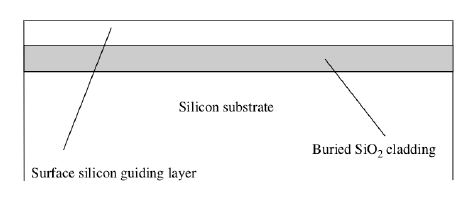
\includegraphics[width = .7\textwidth]{img/SOIstructure}
\caption{SOI chip layer structure}
\label{SOIstructure}
\end{figure}
\\The most important block for a optical chip is a waveguide. The signal is carried inside this block by confinement of light. Consider the system in figure \ref{criticalangle}, when the light strikes the medium boundary, a part is reflected, while another part is transmitted. If the angle of incident $\theta_I$ is less than a critical angle $\theta_c$, the light is completly reflected. Indeed, the angle of the refracted light is given by the snell's law
\begin{equation}n_1 \sin \theta_I = n_2 \sin \theta_T\end{equation}
which can be written as
\begin{equation}\sin \theta_I = \frac{n_1}{n_2}\sin \theta_R\end{equation}
if we impose $\theta_R$ to be at least $90\degree$, we obtain
\begin{equation}\sin \theta_I = \frac{n_1}{n_2} \implies \theta_I = \arcsin\left(\frac{n_1}{n_2}\right) \end{equation}
this is the critical angle, it's clear from the equation that the critical angles exist only if $n_1/n_2<1$, i.e. $n_1>n_2$. Hence the phenomenon of total internal reflection occurs only when light is inside a medium with a refractive index greater than the surrounding's. This is the case of SOI device, where the light propagates inside a layer of silicon sandwiched between a layer of silica and the air which have a refractive index smaller than the silicon's.\\
Inside a waveguide, several modes of propagation are possible, the electric field profile $E_m$ follows the Helmoltz equation:
\begin{equation}(\nabla_{xy}^2 + \beta_m)E_m(x,y)= \frac{\omega^2}{c^2}n^2E_m(x,y)\end{equation}
where $\beta_m$ is called the modal propagation costant, and it's given by $\beta_m = \frac{\omega}{c}n_{eff}$ where $n_{eff}$ is the effective index. $m$ is an integer that represent the discrete mode of propagation.
\begin{figure}
\centering
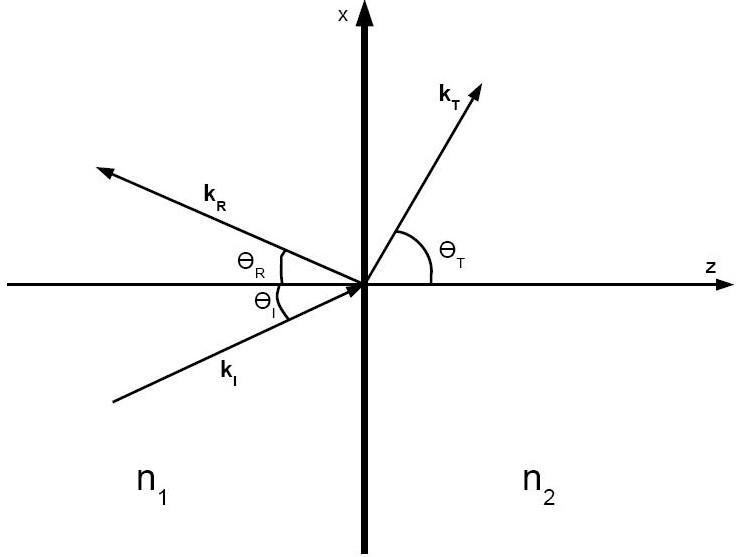
\includegraphics[width = .5\textwidth]{img/TIRDiagram3}
\caption{Light behaviour at media boundary}
\label{criticalangle}
\end{figure}

An important physical conseguence can be deduced from this equation, the electric and the magnetic field cannot be discontinuos at the boundary, so the field is not totally inside the waveguide, but a small part can be found also outside. Indeed Maxwell's equations impose boundary conditions on the electric and magnetic field, the solution of those equations outside the waveguide must be vanishing and it cannot transport energy, otherwise the light would not be confined inside the waveguide, the only solution is to have a exponentially decreasing wave that is called the evanescent wave. This evanescent wave explain why there is the effective index in the formula of the modal propagation costant, the wave, which travels inside the waveguide, propagates inside a medium with fixed refractive index and its tail propagates outside the waveguide where there is a different refractive index, the effective index accounts for this phenomenum.
Evanescent field are also important when two waveguides are really close to each other, if light travel inside a waveguides and its evanescent tail reaches the neighbourn waveguide there is transfer of energy and the light can penetrate into the core of the neighboring one. This allows the coupling of different waveguides or, as we'll see later, the coupling between a waveguide and a resonator. It's also interesting to look at the quantum description of this effect, a photon is described by a wave function which is a solution of the Schr{\"o}dinger equation, in the same Mathematical way of the maxwell's equations, this impose the continuity of the wavefunction across the medium bondary. If two waveguides are close enough, the wave function is non zero inside both waveguides, so a photon have a non zero probability to pass through the gap and change waveguide, in quantum mechanics this effect is called quantum tunneling. 
\section{Resonator}
\begin{figure}
\centering
\begin{subfigure}{0.5\textwidth}
\centering
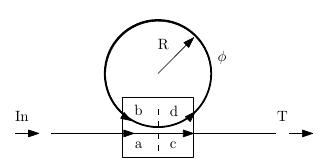
\includegraphics[width = \textwidth]{img/APF}
\caption{}
\end{subfigure}%
\begin{subfigure}{0.5\textwidth}
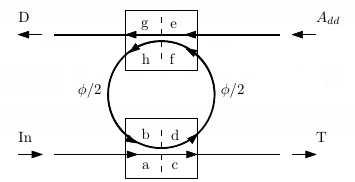
\includegraphics[width = \textwidth]{img/ADF}
\caption{}
\end{subfigure}
\caption{Basic configuration with waveguides and a resonator (a) All Pass Filter (b) Add Drop Filter}\label{basicconfiguration}
\end{figure}

A waveguide can be bended and closed to itself to provide coherent feedback to the circulating light. Such devides is called a resonator and it can have different shape, such as ring, racetrack, disk, toroid. Due to the size of these device they are called microresonator. For the ease of the calculation we'll treat only microrings with fixed radius, typically this radius is in the order of the $\mu m $. Inside a ring resonator light interferes constructively if it's satisfied $n_{eff} L = m \lambda_m$, where L is the lenght of the circumference, $m$ an integer and $\lambda_m$ is the light wavelenght. A consequence of constructive interference is that inside the resonator a large amount of energy is stored and the intesity of the field is enhanced. A strong electric field can cause non linear effects, this is a reason on the importance of resonators, with low power input it's possible to have non linear effects that usually require more powerful source. Ring resonators have a lot of applications, for example they can be used as filter for specific wavelengths for multiplexing applications, sensing, signal modulation and active device for building integrated microlaser.\\
There are mainly two ways to create circuts with the two basic blocks just described, the first one is a waveguide side coupled to a single ring, this configuration is called All Pass Filter (APF), while if there are two waveguide coupled to a single ring, the configuration is called Add-Drop Filter (ADF). In figure \ref{basicconfiguration} we can see both configurations. The coupling is possible by means of the evanescent wave, since the gap between the waveguide and the ring is really narrow (order of $\simeq 100\, nm$).\\
Coupling can be seen as a quad port beam splitter and the relationship between the complex amplitudes of waves in input and output can be represented with the following matrix
\begin{equation}M = \begin{pmatrix}
r & ik \\
ik & r\\
\end{pmatrix}\end{equation}
where $r$ is the reflection coefficient and $k$ is the transmission coefficient, they satisfy $r^2 +k^2 = 1$. The elements of the matrix can be found imposing energy conservation among input and output \cite{thesis:masi}. Let's focus now on the APF configuration, using the the above matrix we want to find the relation bewteen $a$ and $c$ in order to find the transfer function of the device
\begin{equation}\label{APF}\begin{pmatrix}c \\ d \end{pmatrix} = M \begin{pmatrix}a\\b \end{pmatrix}\end{equation}
$b$ and $d$ are connected with the roundtrip phase condition $b = e^{-\alpha 2\pi R} e^{-i\beta 2\pi R}d \equiv\tau e^{-i\phi(\lambda)}d $, in wich $\alpha$ is the linear absorption coefficient, $R$ the ring radius and $\beta$ is the bent mode wavevector $\beta = \frac{2\pi n_{eff}}{\lambda}$. Solving the system \eqref{APF} leads to the transfer function
\begin{equation}H_{AP} = \frac{c}{a} = \frac{\tau - re^{i\phi(\lambda)}}{r\tau -e^{i\phi(\lambda)}}\end{equation}
for the ADF configuration, the expression of the transfer function can be obtained in a similar way, but now we need to handle two beam splitter, and the round phase condition are more complicated: $f = e^{-\alpha \pi R} e^{-i\beta \pi R}d$ and $b=e^{-\alpha \pi R} e^{-i\beta \pi R}h$, working out the calculation we get the final result
\begin{equation}H^D_{AD} = \frac{c}{a} = \frac{k^2\sqrt{\tau} e^{i\phi/2}}{r^2\tau -e^{i\phi}}\qquad H^T_{AD} = \frac{g}{a} = \frac{r(e^{i\phi} - \tau)}{e^{i\phi}-r^2\tau} \end{equation}
another important is the quality factor $Q = \frac{\lambda}{\Delta \lambda}$, where $\Delta \lambda$ is the full width at half maximum of the lorentzian resonance at wavelenght $\lambda$. Equivalently the quality factor can be seen as the ratio between the stored energy inside the cavity and the amount lost per cycle. Futhermore the quality factor is directly correlated with the enhancement factor $EF$ which is the ratio between the amplitude of the electric field inside the resonator and the exciting electric field. An expression for the quality factor can be obtained by taking two successive resonance and calculating the free spectral range, with a Taylor expansion it can be found \cite{thesis:borghi} for the APF and ADF configurations
\begin{equation}
Q_{APF} = \frac{\pi n_g \lambda_m 2\pi R \sqrt{r\tau}}{(1-r\tau)\lambda_m} \qquad Q_{ADF} = \frac{\pi n_g \lambda_m 2\pi R r\sqrt{\tau}}{(1-r^2\tau)\lambda_m}
\end{equation}
from this equation we can see that it's possible to achive high quality factor with large rings and low losses. For example with losses in the order of $< 0.05 \frac{dB}{90\degree}$ and a radius of $< 2\mu m$ the quality factor is up to $10^5$.
\section{Coupled resonators} 
A more interesting configuration of microresonators is presented in figure \ref{resonatorcoupled}. The configuration is composed by two ADF connected in series and it is the configuration on which this work is based. Between the microresonators there is an heater that by heating up the waveguide is able to change the phase of the field travelling inside the waveguide. The idea is that in general the generated photons can exit both from T, both from D or one photon in T and one photon in D, but, by changing the phase $\phi_1$ and $\phi_2$, it is possible to decide where the photons exit. A useful quantity that will need in this work is the field enhancement of the rings. The analytic expression can be found using the formalism developed in the previous section, and the results are
\[FE_1 = \frac{ie^{i(\varphi_1+\phi_2+\phi_1)}k (e^{i\varphi_2}-r^2\tau_2)-ie^{\frac{i}{2}(\varphi_1+\varphi_2)}k^3(k^2+r^2)\sqrt{\tau_1\tau_2}\tau L^2}{e^{i(\phi_1+\phi_2)}(e^{i\varphi_1}-r^2\tau_1)(e^{i\varphi_2}-r^2\tau_2)-e^{\frac{i}{2}(\varphi_1+\varphi_2)}k^4\sqrt{\tau_1\tau_2}\tau L^2}\]
\[FE_2 = \frac{ie^{i(\varphi_2+\phi_1)}kr (-e^{i\varphi_1}+(r^2+k^2)\tau_1)\tau L}{e^{i(\phi_1+\phi_2)}(e^{i\varphi_1}-r^2\tau_1)(-e^{i\varphi_2}+r^2\tau_2)+e^{\frac{i}{2}(\varphi_1+\varphi_2)}k^4\sqrt{\tau_1\tau_2}\tau L^2}\]
where the number 1 refers to the ring on the left and the number 2 to the ring on the right, $\varphi = \beta L$ where $L=2\pi R$. Figure \ref{FE} shows field enhancements in the case of $\phi_1 + \phi_2 = 2m\pi$ around the pump wavelenght. The condition $\phi_1 + \phi_2 = 2m\pi$ is important because it enhances the optical power inside the ring and split, as can be seen from the figure, the energy equally between the two rings. An equally splitted energy means that the two rings are indistinguishable and therefore there is the same probability that the photons are generated inside one or in the other ring. Indeed, if the energy is not splitted equally, it means that only one ring works and the configuration is identical to a simple ADF, hence the tuning with the heaters won't work. 
\begin{figure}
\centering
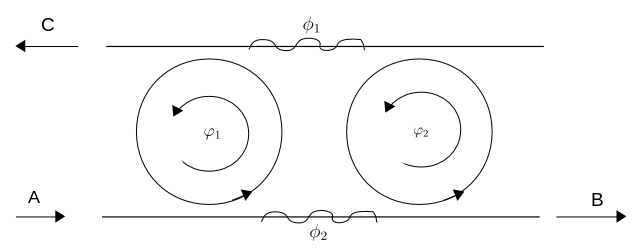
\includegraphics[width = .7\textwidth]{img/coupled}
\caption{Two resonators coupled togheter}
\label{resonatorcoupled}
\end{figure}

\begin{figure}
\centering
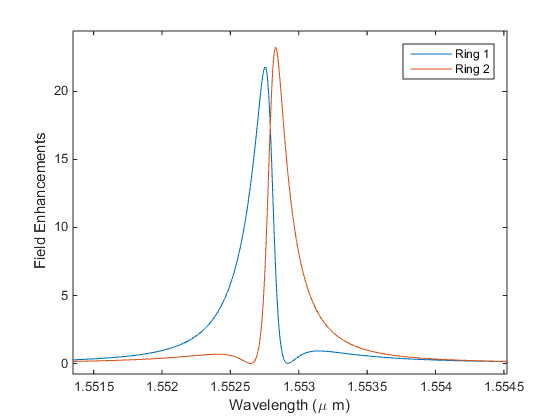
\includegraphics[width = .8\textwidth]{img/FE_fase_2pi}
\caption{Field enhancements with $\phi_1+\phi_2 = 2\pi$, ring 1 refers to the left one and 2 to the right one}
\label{FE}
\end{figure}